%!TEX root = bare_conf.tex

\section{Approach}\label{sec:approach}

In order to solve the task of autonomous driving in the simulation environment we had to make some fundamental decisions. First of all we specified our input source.The image of a front facing camera was chosen as input, because it provides more than enough information for this task. Secondly we decided to use an action set of five actions including straight, left, right, half left and half right. The angles of left and right were chosen that the car can easily complete every curve. The actions and their values are listed in \ref{woauchimmer}. To support the mentioned input and generate the required output the given network was altered as described in the following section.

\subsection{Network}
The network we use is based on the one introduced by Mnih et al. \cite{Mnih13}. Instead of four frames we process only one frame at a time, because lane following at constant speed does not require temporal context. The size of the input image is reduced to 48 $\times$ 27. At this resolution the camera image still contains enough information on the lane markings. The network has two convolution layers and two fully connected layers. Both convolutional layers use 4 $\times$ 4 kernels with a stride of 2. Layer one learns 16 filters, while layer two learns 32. The first fully connected layer has 256 neurons. The second fully connected layer computes 5 outputs, which represent the Q value for each action.

%-Structure + Parameters
%-Input
%-Output / Actions

\subsection{Training}
The framework used for training is an implementation of the paper ''Playing Atari with Deep Reinforcement Learning``  created by Peter Wolf. We altered some training parameters to adapt the framework to our needs. Therefore we set the size of the replay memory to 500k, in order to use the maximum memory available on the machine which was 16GB. The exploration value varied from 2 million Iterations up to 5 million, depending on the estimated training complexity. We also limit the length of an episode to 10k actions, to ensure a valid position of the car. An episode may end before reaching this limit, if the car leaves the driving lane. At the beginning of each episode the car is randomly placed on the track. This is done to ensure the entire track gets explored early on.

In training the weights of the network are adjusted every iteration. By default the simulation continues while updating the weights. To avoid frame skips in training that are not present while evaluating, we decided to pause the simulation while updating the weights.

For the network an initial learning rate of $10^{-5}$ is chosen, which is decreased by a factor of 0.1 every 2 million iterations.

These settings allowed us to complete 3 to 4 million iterations per day. The plots in figure \ref{fig:lossandrew} show that the training is finished after 6 million iterations. That means that approximately 48 hours of training are needed every time a change is made.

\begin{figure}[!t]
\centering
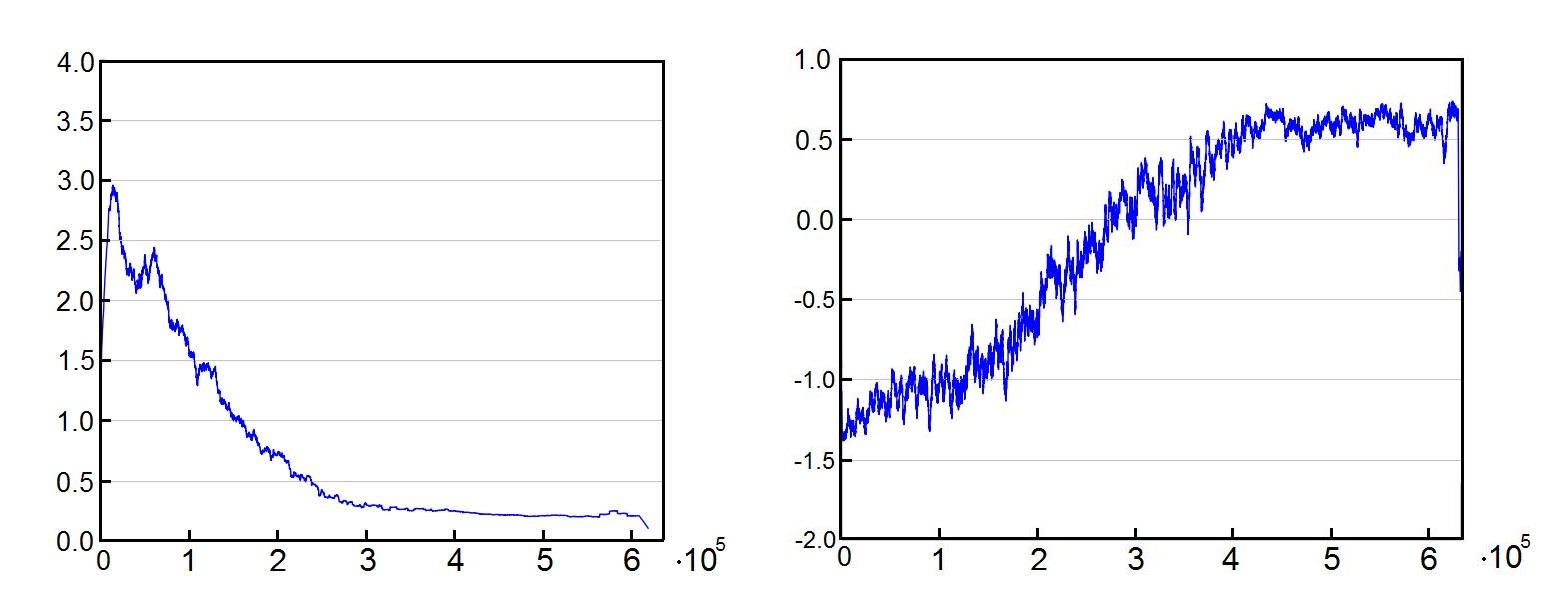
\includegraphics[width=3.5in]{../presentation/both-plot.jpg} 
\caption{Left: Loss of the network for one training. Right: Reward collected by the car. After approximately 4 million iterations both values are converged.}
\label{fig:lossandrew}
\end{figure}
 
%-Trainings params
%-Performance 
%-Pause physics
%-Loss + Reward plots

\subsection{Reward function}
The behaviour of the car is controlled through the reward function, hence any changes need to be done advisedly. As soon as the framework was up and running almost the entire development time was designated for testing of various functions. 

To ease development we decided to display a color coding of the current reward directly on the vehicle. This allowed us to check, before launching a new training, if the changes made to the reward function promised noteworthy gains or if they contained any errors. 
%-to ease development of reward function -> coloring
%-plot distance 
\subsubsection{Distance based}
A distance function serves as an intuitive starting point to teach the car where it is currently located in relation to the road. There are several problems with this simple approach though. The current distance is not a result of the currently chosen action, but the one of the past actions up to this point. While Q-learning methods do account for this, having a delayed reward does drag out the training time. Furthermore there is no feedback concerning the cars orientation in relation to the road. This can result in good rewards even though the car is arbitrarily oriented. As a consequence driving behaviour will be anything but smooth.
%-Reward lacks immediate feedback
\subsubsection{Distance and Action based}
To tackle the lack of immediate feedback we used several action assessments. Depending on the current state, some actions can only be decremental and should therefore be punished while others may be beneficial and should be rewarded. One important thing to note here is to handle the balance between distance and action based rewards with care. If one is weighted too heavily, the other one might get ignored, resulting in a performance decrease.

First we added a punishment if the car was on one side of the road, oriented away from it and also steering away from it. While this might be a useful action for advanced tasks, it is not at any time helpful to stay in the lane.

Next was optimizing the behaviour on a straight road. We give an additional reward if the car is located on a straight road, is in proximity to the center of the lane and chooses to steer straight.

Lastly we punished countersteering in curves. While human drivers often do exploit this to stay in lane, we hoped for a smoother result if the car made less use of it.